%%
\documentclass{abnt}
% Incluir Pacotes ------------------------------------------------
\usepackage [brazil] {babel}
\usepackage [utf8] {inputenc}
\usepackage{ae}                  %% Font Encoding T1 (PDF)
\usepackage{graphicx}            %% Incluso de grficos (DVI/PS)
\usepackage{geometry}            %% Dimenses do documento (DVI/PS)
\usepackage{lscape}              %% Utilizar pgina em landscape
\usepackage{url}                 %% Trata URLs, e-mails e paths
\usepackage[alf]{abntcite}
\usepackage{listings}
\usepackage{color}
\usepackage{amssymb}
%\usepackage{float}


\renewcommand{\ABNTchapterfont}{\fontfamily{cmr}\fontseries{b}\selectfont}
\renewcommand{\ABNTsectionfont}{\fontfamily{cmr}\fontseries{b}}
\renewcommand{\tituloformat}{\large\bfseries}

\begin{document}
% ----------------------------------------------------------------
% Paginas iniciais
% ----------------------------------------------------------------
% \autor{Antonio Ribeiro Alves Júnior}

\titulo{Arquitetura de um Middleware para Simulação Distribuída}

\comentario{Dissertação submetida ao Programa de PósGraduação em Ciência e Tecnologia da Computação como parte dos requisitos para obtenção do Título de Mestre em Ciência e Tecnologia da Computação.}

\instituicao{Universidade Federal de Itajubá - Unifei \par Instituto
de Engenharia de Sistemas e Tecnologias da Informação Engenharia da Computação}

\orientador{Prof. Dr. Edmilson Marmo Moreira}

\local{Itajubá - MG}

\data{01 de Junho de 2012}

\capa

\folhaderosto                    %% Capa e Folha de rosto
\tableofcontents                  %% Sumário
\listoffigures                    %% Lista de figuras
% \chapter*{Agradecimentos}

Acima de tudo agradeço a Deus.

Agradeço ao professor Dr. Edmilson Marmo Moreira que, além de me apoiar e me orientar, me suportou durante esses vinte meses de trabalho, incluindo duas mudançaas de cidade.

À Minha esposa Gislene, companheira de todos os momentos e incentivadora maior do meu trabalho.

Aos meus pais, Antonio e Márcia, pelo indubtável apoio em todos esses anos de Unifei.

Aos amigos e companheiros de república Maurício Faria, Gustavo Walbon e Tiago Maluta, que foram fontes de inspiração na minha jornada acadêmica. A computação não seria tão interessante e divertida se não fosse a companhia de vocês.

\textit{Antonio Ribeiro Alves Júnior}
          %% Agradecimentos
%-----------------------------------------------------------------
% Corpo da Monografia
% ----------------------------------------------------------------
\chapter{Introdução}
\section{Simulação}

A simulação é uma técnica que permite prever e visualizar o comportamento de sistemas reais a partir de modelos matemáticos. As aplicações da simulação abrangem diversos benefícios, tais como: a possibilidade de antever possíveis problemas ou comportamentos indesejáveis de um sistema, auxílio na tomada de decisão sem a necessidade de intervir no sistema real, facilidade na manipulação e alteração dos modelos, economia de recursos (físicos e financeiros) durante a tomada de decisões, dentre outros.

Para utilizar a simulação é necessário construir e analisar modelos que represente o sistema. Os modelos podem ser classificados de diferentes formas. Uma classificação pode ser considerada verificando a influência ou não de variáveis aleatórias no sistema. Os sistemas são ser representados por um modelo determinístico, quando estes podem ser considerado totalmente livre de aleatoriedade, ou estocásticos, quando estes consideram aleatoriedade.

Os modelos que descrevem o comportamento através do tempo podem ser classificados como contínuos e discretos no tempo. Nos modelos de estados contínuos, as variáveis de estados variam espontaneamente. Já nos modelos de estados discretos, as mudanças ocorrem em pontos específicos e descontínuos do tempo.

Este trabalho enfoca os modelos estocásticos e de estados discretos, uma vez que eles são os que melhor representam modelos de sistemas computacionais.

Um sistemas de simulação sequencial, onde uma única máquina executa toda a simulação, pode ser retratado como uma fila de eventos aguardando para serem tratados. Cada evento possui o seu tempo de execução, como pode ser visto na figura~\ref{fig:simul}, que deve ser obedecido para garantir consistência do resultado.

Neste modelo sequencial, o sistema responsável pela simulação retira o próximo evento da fila de execução para tratá-lo. Ao fim do processamento, um próximo evento é retirado da fila, e isto se repete até o final de lista de eventos futuros. O tratamento de um evento pode ou não resultar dados que sejam necessários em um processamento futuro.

\begin{figure}
  \centerline{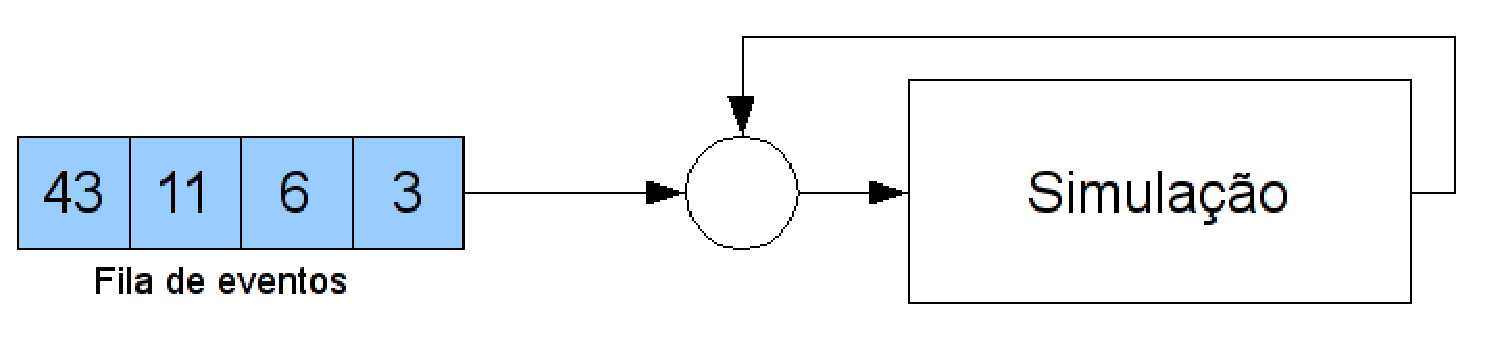
\includegraphics[scale=0.6]{simulacao.eps}}
  \caption{Simulação Sequencial.}
\label{fig:simul}
\end{figure}

\section{Simulação Distribuída}
A simulação é um processo que apresenta um custo computacional muito alto, tendo em vista a grande quantidade de dados que devem ser processados e a complexidade dos modelos matemáticos empregados. Esses fatores em conjunto podem encarecer computacionalmente o sistema, levando à ineficiência da simulação.

Uma das formas encontradas para se solucionar estes problemas foi dividir o tratamento dos diversos eventos entre vários processadores de uma mesma máquina paralela ou sobre um sistema distribuído, dando origem assim à Simulação Distribuída.

Distribuindo os eventos, reduz-se o tempo gasto pelos programas de simulação, mas, em contrapartida, novas situações necessitam de observação devido às características deste tipo de aplicação. É preciso sanar os problemas com a sincronização dos processos, sobrecarga da rede de comunicação, necessidade de balanceamento de carga do sistema, dentre outros.

Em um sistema de Simulação Distribuída, três estruturas devem ser observadas no desenvolvimento da simulação orientada à eventos:

\begin{itemize}
    \item As variáveis que descrevem os estados do sistema;
    \item Uma lista de eventos futuros, que contém os eventos a serem executados;
    \item Um relógio Global, que controla o progresso da simulação.
\end{itemize}

Os eventos devem ser executados obedecendo o seu \textit{timestamp}. O programa de simulação deve remover repetidamente da fila o evento com a menor marca de tempo e executá-lo. Assim que um evento é retirado da fila de execução, o relógio global avança para o tempo de ocorrência do evento. Esse mecanismo garante que todos os eventos sejam executados obedecendo a ordem cronológica do tempo de simulação. Porém, em se tratando de um sistema distribuído, não há como haver uma fila única de eventos. Portanto, o sistema passa a ser dividido em $n$ processos denominados $p_{1}, p_{2},\ldots, p_{n}$, cada um representando um processo do sistema real. Novos mecanismos devem ser incorporados ao sistema de simulação para garantir que cada evento seja executado na sua devida ordem.

Para cada processo lógico é atribuído um relógio que indica o seu progresso na simulação. A comunicação entre os processos se dá através mensagens, uma vez que não há áreas de memória compartilhadas entre os processos. Estas mensagens são também responsáveis pela sincronização do sistema. Caso algum evento $e_b$ venha a ocorrer antes de um segundo evento $e_a$, e sendo $a < b$, tem-se assim um erro de causa e efeito. Como em um sistema real nunca existirá tal situação, isto caracteriza uma inconsistência na simulação.

Os conceitos de sincronização de processos levaram ao desenvolvimento de protocolos, classificados como conservativos ou otimistas, para garantir a sincronização dos processos da simulação distribuída, evitando ou corrigindo erros de causa e efeito \cite{FUJIMOTO}.

\section{Objetivos}
Este trabalho tem como objetivo avaliar a viabilidade de se implementar um protocolo de sincronização de simulação distribuída utilizando agentes móveis. Para isto é empregada a utilização da biblioteca de agentes móveis \textit{Aglets} para a implementação do protocolo \textit{Rollback} Solidário.

\section{Organização da Monografia}
Os capítulos seguintes abordam uma leve explicação do funcionamento dos protocolos de sincronização de simulação distribuída e de como o trabalho foi abordado para a sua implementação.

O capítulo dois trata dos protocolos de sincronização de eventos em simulação distribuída. Ele inicia com a explicação das principais diferenças entre protocolos conservativos e otimistas, e em seguida traz o princípio básico de funcionamento dos protocolos \textit{Time Warp} e \textit{Rollback} Solidário.

No terceiro capítulo são apresentados os agentes móveis e a biblioteca \textit{Aglets}, assim como o seu funcionamento no contexto computacional.

O quarto capítulo trata a implementação do protocolo \textit{Rollback} Solidário sobre a biblioteca \textit{Aglets}, assim como o seu funcionamento.

Por fim, o capítulo número cinco discute as conclusões obtidas e as possibilidades de continuação deste trabalho.              %% 1 INTRODUÇÃO
\chapter{Simulação Distribuída de Eventos Discretos}

Parágrafo 1: Revisar a déia inicial sobre o que é simulação, e dizer que a simulação é baseada em um modelo do problema

Parágrafo 2: Dizer que a simulação é um processo caro, e que é conveniente dividir entre vários computadores (distribuir a simulação)

Parágrafo 3: Apresentar problemas como sincronização, comunicação, balanceamento de cargas, etc. devido à distribuição.

Parágrafo 4: Dividir o sistema em Processo lógicos e eventos discretos. Rever o conceito de timestamp de cada evento.

Parágrafo 5: Dizer que cada processo lógico possui um relógio interno

Parágrafo 6: Definir comunicação através de troca de mensagens

Parágrafo 7: Definir o conceito de sincronização (timestamp das mensagens e LVT)


\section{Categorias de protocolos de simulação}

Parágrafo 1: breve discussão sobre as categorias de protocolos, explicando as principais diferenças

\subsection{Protocolos conservaticos}

Parágrafo 1: citar Srinivasan and Reynolds, explicando o conceito básico de um protocolo conservativo

Parágrafo 2: citar as implementacoes de [chandy e misra] e bryant, citando a necesidade de canais estaticos

Parágrafo 3: citar problema de bloqueio por esperar mensagem que contém um lvt inferior, citar também como contornar esse deadlock

Parágrafo 4: explicar porque é difícil resolver o problema de deadlock

Parágrafo 5: citar a desvantagem do conservativo por não aproveitar todo o paralelismo

Parágrafo 6: conclusão pessoal de porque não utilizar o protocolos conservativos

\subsection{Protocolos Otimistas}

Parágrafo 1: explicação inicial do conceito de protocolo otimista e citar o conceito de rollback

Parágrafo 2: Citar o time warp, contextualizando como foi desenvolvido, em qual época e por quem

Parágrafo 4: Citar o Rollback Solidário como alternativa ao Time Warp

\section{O protocolo \textit{Time Warp}}

Parágrafo 1: Explica por que o Time Warp é otimista, citando o fato de nao impedir a ocorrência de erros de causa e efeito

Parágrafo 2: Citar como um erro de causa e efeito pode acontecer, e o que deve ser feito quando isso acontece: o rollback

Parágrafo 4: Citar implementações do protocolo

Parágrafo 5: Explicar o comportamento individual de um processo lógico (tirar o eventos com menor timestamp da lista de eventos futuros, etc.)

\subsection{Detecção e Tratamento de Inconsistências}

Parágrafo 1: Mostrar que o sistema pode receber mensagens que causam erro de causa e efeito.

Parágrafo 2: Explicar o comportamento ao receber uma mensagem straggler.

Parágrafo 3: definir a diferença entre rollback primário e rollback secundário

\subsection{Anti-Mensagens}

Parágrafo 1: Explicar o que é uma antimensagem

Parágrafo 2: mostrar que antimensagens podem se referir a um evento já processado, ou a um evento que ainda esta na fila de eventos futuros

Parágrafo 3: Tratar o caso da antimensagem chegar antes da mensagem

\subsection{Considerações Finais}


\section{O protocolo \textit{Rollback} Solidário}

Parágrafo 1: Apresentar a principal diferença do rollback solidário

Parágrafo 2: explicar que, em caso de erro de causa e efeito, todos os processos executam rollback em conjunto

Parágrafo 3: introduzir o conceito de checkpoint, checkpoint global e checkpoint local.

\subsection{Comportamento Geral do Protocolo Rollback solidário}

Trazer uma idéia básica do Rollback solidário em linhas gerais

\subsection{Estados Locais e Estados Globais}

Parágrafo 1: Definição de um estado local como sendo os valores das variáveis do processo em questão em um determinado tempo

Parágrafo 2: Definição de estado global como sendo um conjunto de estdaos de cada processo.

\subsection{Cortes Globais Consistentes}

Parágrafo 1: Apresentar o conceito de precedência causal

Parágrafo 2: Definir corte 

Parágrafo 3: definir corte consistente utilizando precedência causal

\subsection{Relógios Lógicos e Relógios Vetoriais}

Parágrafo 1: Apresentar o conceito de relógio lógico

Parágrafo 2: Mostrar que o relógio lógico não representa a precedência causal em um sistema distribuído

Parágrafo 3: Apresentar o conceito de relógio vetorial

\subsection{Checkpoints Globais Consistentes}

Parágrafo 1: Definir o que é um checkpoint: um ponto de retorno que foi, de alguma forma, armazenado de forma persistente

Parágrafo 2: a necessidade de se garantir que um checkpoint seja consistente

Parágrafo 3: associação de checkpoint consistente com corte consistente

\subsection{Obtenção de Checkpoint Semi-Síncrono}

Parágrafo: introduzir o processo observador

Parágrafo: Introduzir o vetor de dependência

Parágrafo: Mostrar como a troca de mensagem deve levar o vetor de dependências, e como este deve ser atualizado no processo que recebeu a mensagem

Parágrafo: mostrar como o processo observador monta uma linha de recuperação através da matriz de dependências

Parágrafo: demonstrar que um checkpoint global consistente é formado por checkpoints locais que não possuem relação causal entre si


\subsection{Tratamento dos Rollbacks na Abordagem Semi-Síncrona}

Parágrafo: Explicar o comportamento de um processo ao receber uma mensagem straggler 

Parágrafo: Falar sobre a atuação do processo observador (escolher a linha de retorno, avisar o rollback à todos em broadcast, etc.)

Parágrafo: Falar sobre o reinício da simulação após o Rollback

\subsection{Considerações Finais}


\section{Balanceamento de cargas}

Parágrafo: apresentar o balanceamento de carga como fator determinante no desempenho de uma simulação distribuída

Parágrafo: Introduzir o conceito de escalonamento de processos como meio de prover o balanceamento de cargas

Parágrafo: por fim mostrar que para prover o balanceamento de cargas temos que possibilitar que um processo lógico migre de um nó do sistema para outro

\subsection{O Uso de Agentes Móveis Para Prover Mobilidade}

Parágrafo: O que é um agente móvel

Parágrafo: Falar sobre a implementação feita por Antonio, Walbon e Takahashi - 2010

Parágrafo: Outras implementações feitas usando agentes móveis

\subsection{Requisitos Para Mobilidade de um Processo Lógico}

Parágrafo: explicar quais as funcionalidades de agentes móveis que precisamos (migração)

Parágrafo: Abstrair o conceito de ambiente e processo lógico: um ambiente abriga diversos processos lógicos

Parágrafo: Mostrar a idéia de migrar um processo de um ambiente para outro, a fim de prover o balanceamento

\subsection{Considerações Finais}
           %% 2 Simulação Distribuída
\chapter{Proposta deste projeto}

Neste capítulo pretende-se apresentar a proposta de uma arquitetura que visa sustentar o desenvolvimento de aplicações de simulação distribuída de maneira transparente para o usuário final. Em complemento é trazido também neste capítulo algumas soluções já existentes e, por fim, pretende-se defender a proposta de se optar por uma nova arquitetura de comunicação entre processos lógicos.

\section{Um \textit{framework} para simulação distribuída}

Escrever uma aplicação de simulação de eventos discretos distribuída é uma tarefa de grandes proporções. Todo o tratamento de sincronização, comunicação, troca de mensagens, manipulação de objetos remotos, dentre outros, acarretam na existência de diversas tarefas paralelas à simulação em si, que devem ser gerenciadas pelo desenvolvedor que pretende implementar a simulação.

Some-se a isso questões de ordem prática, como cuidado com o desempenho (entram neste ítem balanceamento de carga, \textit{design} eficiente dos algorítmos utilizados, etc) e permissividade ao erro (a probabilidade de se intruduzir um erro em um código aumente proporcionalmente ao tamanho deste código, \cite{HONGYU09}). Obtemos neste ponto um cenário onde o desenvolvedor acaba tendo de se ater a diversos detalhes alheios à simulação propriamente dita, que torna impraticável um desenvolvimento sustentável de simulações distribuídas.

Assim como proposto em \cite{LIVERSON}, um framework de simulação distribuída tem o objetivo de suportar o desenvolvimento de simulações distribuídas de uma maneira que proveja encapsulamento dos mecanismos alheios à modelagem e execução da simulação, transparência nas tomadas de decisões internas e reusabilidade de código.

\subsection{Encapsulamento}

Uma das funções de um \textit{framework} é o de encapsular diversos elementos que não tratam diretamente da simulação, mas sim sustentam funcionalidades que dão vida à simulação propriamente dita. Exemplo disso é a possibilidade de se criar elementos lógicos para compor o modelo, análogos à componentes em um circuito elétrico. Encapsulando o funcionamento de uma fila ou o de um processo consumidor em uma classe por exemplo estamos isolando sua implementação e seus detalhes do usuário final do \textit{framework}. A este usuário cabe reutilizar estes componentes e, quando julgar necessário, criar componentes baseados nesses primitivos.

Outro ocasião em que pode-se aplicar o encapsulamento é tanto nos algorítmos responsáveis pelo balanceamento de cargas no sisteam quanto nos mecanismos de sincronização de processos lógicos. A possibilidade de encapsular esses componentes do framework em classes separadas nos possibilita o intercâmbio de diferentes implementações que solucionam um mesmo problema. Com uma interface bem desenvolvida, pode se criar, por exemplo, encapsulamentos distintos para o protocolo \textit{Time Warp} e para o protocolo \textit{Rollback} Solidário. Isso permitiria que o usuário escolhesse, antes de iniciar a simulação, qual protocolo pretende adotar no processo.

\subsection{Transparência}

A proposta de se escrever um código que seja ao mesmo tempo fácil de se implementar pelo usuário e eficiente em sua execução projeta-se diretamente na utilização de diversas camadas que ao mesmo tempo esconde do usuário do \textit{framework} algumas decisões internas e provê abstrações nas quais o usuário se baseia para desenvolver seu modelo.

Segundo \cite{DIRK00}, um usuário ao utilizar um \textit{framework} reutiliza seu \textit{design} e sua implementação. Isto é feito pois cabe ao framework resolver os problemas referentes ao seu domínio (no caso proposto por esse trabalho: sincronismo, comunicação, migração e balanceamento de carga em um sistema distribuído de simulação), deixando ao usuário apenas a função de desenvolver a aplicação sem a necessidade de se preocupar com questões que estão fora de seu domínio.

O conceito de transparência neste caso remete-se que a intenção do \textit{framework} é deixar invisível ao seu usuário toda e qualquer decisão que não compete à construção do seu modelo a ser simulado. Isso acaba trazendo para a construção do \textit{framework} algumas responsabilidades quanto a tomadas de decisões sobre \textit{design} de software, implementação de algorítmos considerados decisivos, entre outros.

\subsection{Reusabilidade}

Ao se optar pelo desenvolvimento de um \textit{framework} o responsável pelo seu \textit{design} deve permitir que componentes de interesse sejam trocados ou mesmo customizados. Isso faz com que que o mesmo código escrito para um framework funcione mesmo depois da troca de algum componente deste framework.

No caso da simulação distribuída, componentes como protocolo de sincronização ou sistema de balanceamento de cargas poderiam ser plugáveis, o que permitiria a reutilização do mesmo código de simulação no mesmo framework, porém com caracterúisticas diferentes. Isso leva à uma reutilização de código, economizando no desenvolvimento e dinamizando a comparação entre diferentes soluções para um mesmo modelo.

\section{Soluções Existentes \label{solucoes_existentes}}

Uma proposta de \textit{framework} para simulação distribuída foi proposta em \cite{LIVERSON}, baseada em troca de mensagens suportando tanto \textit{MPI} qaunto \textit{PVM} e abordando tanto os protocolos de sincronização \textit{Rollback} Solidário e \textit{Time Warp}. Em \cite{RIBEIROALVES} é proposto uma solução utilizando agentes móveis, o que contempla, além da comunicação por troca de mensagens, também a possibilidade de migrações de processos lógicos através dos nós do sistema distribuído, visando a possibilidade de balancear a carga entre os nós do sistema.

Algumas propostas como a \textit{Remote Call Framework (RCF)}, \textit{ClassdescMP} e diversas implementações do \textit{MPI} e de \textit{PVM} provém diversas soluções para a a troca de mensagem entre diferentes processos. Essas soluções ao mesmo tempo que provém eficientes mecanismos para gerenciar a troca de mensagens entre os processos, não possuem soluções nativas para a migração de processos lógicos entre nós do sistema de simulação, e também não estão preparados para o redirecionamento de mensagens enviadas à processos que migraram para um nó diferente do seu nó de origem.

Outras soluções como \cite{SASSY} e \cite{}, assim como \cite{RIBEIROALVES} baseia-se nos agentes móveis para se desenvolver a aplicação de simulação distribuída.

Tanto nos casos que utilizam agente quanto nos casos que baseiam-se em suprir soluções para troca de mensagens não é encontrada nativamente todos os mecanismos necessários para a implementação de um sistema de simulação distribuída que suporte tanto troca de mensagem quanto migração de processos. Ao utilizar-se de agentes móveis, que possuem tanto mecanismo de mobilidade quanto mecanismos de troca de mensagens, obtemos em um primeiro momento todos esses elementos. Porém, ao se mover um objeto de um nó para outro, perde-se a referência que havia deste objeto, forçando a se implementar um mecanismo que corrija este cenário. Vale citar também que mecanismos como comunicação grupal, essencial na implementação do \textit{Rollback} Solidário não é compreendido por agentes móveis.

Visando isso este trabalho se propões em apresentar uma solução para se desenvolver simulações distribuídas de eventos discretos que encapsule os macanismos de sincronização de processos, balanceamento de carga, \textit{design} de componentes para a construção do modelo a ser simulado.

Para que seja sustentada tanto os mecanismos de sincronização quanto o balanceamento de carga, é vital que o \textit{framework} supra também as necessidades básicas de comunicação, troca de mensagens, serialização de processos lógicos, migração destes processos e comunicação grupal. Estas funcionalidades são providas pelo \textit{middleware} de comunicação do \textit{framework}. Uma característica fundamental do \textit{middlere} de comunicação proposto por esse trabalho é que, uma vez um objeto migrando de seu nó de origem para um novo local, o \textit{middleware} se encarrega de redirecionar as mensagens destinadas à esse processo lógico em seu novo ambiente, deixando completamente transparente para o usuário questões como endereço físico do processo lógico, \textit{status} do processo, etc.

\section{Arquitetura proposta}

A fim de suprir todas as necessidade de um sistema que suporte plenamente a migração de processos lógicos, é apresentado na~\ref{fig:arquitetura_macro} uma visão bastante ampla da arquitetura do framework de simulação distribuída aqui proposto.

A camada superior, denominada aplicação, é a interface pela qual o usuário do sistema descreve o seu modelo a ser simulado. Cabe ao \textit{framework} prover uma \textit{API} com a qual o usuário descreverá o comportamento do seu modelo.

A camada intermediária compreende tanto os algorítmos responsáveis pelo gerenciamento da simulação (o \textit{kernel} do \textit{framework}) quanto os mecanismos de sincronização e balanceamento de carga. É nesta camada também que se encontra as descrições dos componentes elementares utilizados para a descrição do modelo. São exemplos de componentes: fila, processos consumidor, gerador de eventos, etc.

Por fim, sustentando as demais camadas encontra-se o \textit{middleware} de comunicação. Esta camada é responsável não somente pela troca de mensagens entre processos lógicos, como também por todo o gerenciamento do ciclo de vida de um processo, serialização e migração de processos, reenvio de mensagens para destinatários que migraram, gerenciamento de recursos do sistema e mecanismo de comunicação grupal. 

\begin{figure}
  \centerline{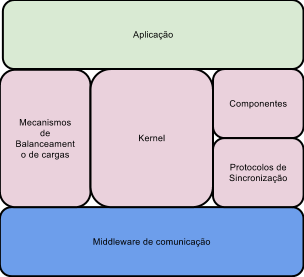
\includegraphics{arquitetura_macro.png}}
  \caption{Camadas da arquitetura do \textit{framework}.}
\label{fig:arquitetura_macro}
\end{figure}

Conforme descrito na seção~\ref{solucoes_existentes}, os mecanismos de troca de mensagens existentes não contemplam nativamente os requisitos que possibilitem tanto a troca de mensagem entre processos e sua migração e, ao mesmo tempo, opere de forma transparente quanto à referenciação de processos lógicos que migraram. Nos casos que mais se aproximam dos requesitos do sistema, os agentes móveis, há uma transparência na troca de mensagens até o momento em que um agente migra para um nó distinto do sistema. Ao se mover para um ambiente diferente do seu ambiente de origem, implementações de agentes móveis como \textit{Aglets} carecem de uma intervenção do usuário para que se refatore os valores dos endereços físicos dos objetos. O middleware aqui proposto visa resolver este problema, tornando a comunicação entre processos completamente transparente para o seu usuário.

\section{Organização deste documento}

Os capítulos seguintes tratam da descrição detalhada da arquitetura do projeto e de sua implementação. O capítulo quatro trata da arquitetura do \textit{middleware} de comunicação. O capítulo cinco traz detalhes da arquitetura do \textit{framework} de simulação.

No capítulo seis é demonstrado detalhes de implementação que o autor julga conveniente explicitar neste documento e no capítulo sete é demonstrado alguns exemplos de simulação utilizando o framework desenvolvido.

Por fim o capítulo oito traz as discussões sobre os resultados desse trabalho, tanto quanto conclusões e propostas para sua continuaidade em trabalhos futuros.

           %% 3 proposta do projeto de mestrado e revisão bibliográfica
\chapter{Arquitetura do \textit{middleware} de comunicação}

Este capítulo descreve em detalhes a arquitetura do proposto \textit{middleware} de comunicação, tais como suas partes e suas principais funções, como troca de mensagens, migração e serialização. 

\section{Componentes do \textit{middleware}}

A arquitetura proposta é dividida em dois componentes principais: o ambiente (\textit{envinonment}) e o processo lógico (\textit{process}). Um ambiente representa um nó lógico do sistema de simulação distribuída, ou seja, é a representação lógica de um computador no sistema distribuído. Em uma simulação distribuída, tipicamente, cada nó físico da rede deve conter um único \textit{environment}.

O segundo componente da estrutura do \textit{middleware}, o processo lógico, que é a representação lógica de um processo no sistema de simulação distribuída. Na arquitetura aqui descrita, um processo lógico somente existe dentro de um \textit{environment}. Sendo assim, um \textit{environment} pode ser visto como um conjunto de processos. Por sua vez, um processo somente pode estar contido por um único \textit{environment} em um determinado momento.

Assim, sendo \textit{p} um processo lógico e \textit{e} um ambiente de simulação contento \textit{n} processos, então definimos:

Definição 1: Um \textit{environment} é um conjunto de processos \begin{equation} e_{k} = \{p_{i} | i < n \} \end{equation}

Definição 2: Um processo só pode estar contido em um único ambiente em um instante bem definido \begin{equation} p_{k} \in e_{l} \rightarrow \not \exists e_{m}, p_{k} \in e_{m}, e_{l} \neq e_{m} \end{equation} 

Tanto o \textit{environment} quanto o \textit{process} são abstrações lógicas que representam a simulação baseado em eventos discretos. Fisicamente tanto o ambiente quanto o processo lógico são instâncias de objetos que devem ser implementadas extendendo classes bases abstratas que contém as especificações descritas por este \textit{middleware}.

A arquitetura do \textit{middleware} aqui proposto deve oferecer as seguintes funcionalidades:
 
\begin{itemize}
\item Comunicação entre processos lógicos por troca de mensagens.
\item Serialização do conteúde de um processo lógico.
\item Migração de um processo de um \textit{environment} para outro.
\item Continuidade da comunicação, de maneira transparente, mesmo após a migração de um processo.
\item Serialização em larga escala de um ambiente ou de toda a simulação.
\item Comunicação grupal entre processos e entre ambientes.
\end{itemize}

A propriedade de comunicação por troca de mensagem é um ítem fundamental para a implementação de simulação distribuída. A forma de se comunicar por troca de mensagens provida pelo \textit{middleware} baseia-se nas quatro suposições iniciais descritas por \cite{MCQUILLAN75} sobre os canais de comunicação inter-processos:

\begin{itemize}
\item O canal introduz um flutuante, porém finito, atraso nas mensagens.
\item O canal possui uma flutuante, porém finita, largura de banda.
\item O canal apresenta uma flutuante, porém finita, taxa de erro.
\item Existe uma real possibilidade de as mensagens transmitidas da fonte para o destino cheguem ao destino em uma ordem diferente da originalmente transmitida. É assumido que tanto a fonte quanto o destino possuem, em geral, finitos tamanhos de \textit{buffers} de armazenamento e diferentes \textit{bandwidth}.
\end{itemize}

A capacidade de um processo lógico migrar de um \textit{environment} para outro é um ponto fundamental para se proporcionar a capacidade de balanceamento de cargas em uma simulação distribuída. O mecanismo de migração, descrito na Seção~\ref{migracao}, é a união da capacidade de serialização de um processo e da comunicação entre diferentes \textit{environments}.

\section{O componente \textit{environment}}

Essencialmente, um ambiente na arquitetura aqui proposta é uma plataforma que abriga e gerencia diversos processos lógicos. A existência desta plataforma como base para o gerenciamento dos processos é justificada quando desejamos manipular simultaneamente características de diversos processos que possuêm em comum o fato de estarem no mesmo ambiente físico (como por exemplo migrar ou serializar todos os processos). Mas principalmente se justifica a existência de uma camada que seja responsável por gerenciar o ciclo de vida de processos, como criação, migração e destruição de processos.

\subsection{Estrutura interna}

Internamente, o \textit{environment} apresenta as seguintes estruturas básicas (conforme ilustrada na Figura~\ref{fig:environment_1}):

\begin{itemize}
\item Estrutura interna de dados do ambiente
\item Tabela de endereços de processos
\item Lista de processos lógicos locais
\item Proxy de comunicação externa
\end{itemize}

\begin{figure}
  \centerline{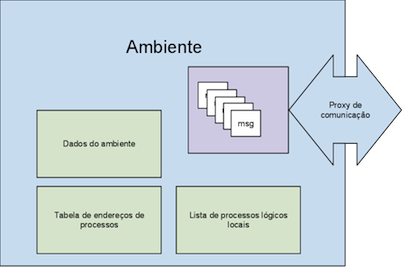
\includegraphics{Environment_1.png}}
  \caption{A arquitetura interna de um \textit{environment}.}
\label{fig:environment_1}
\end{figure}

A estrutura interna de dados do ambiente é a representação de todos as variáveis pertencentes ao \textit{environment}. Dados como o endereço físico (IP) do ambiente na rede, nome lógico do ambiente e quantidade de processos residentes no \textit{environment} são armazenadas neste espaço.

Um \textit{environment} possui um endereço lógico único em toda o ciclo de vida da simulação, denominado \textit{Unique Environment Identifier} - \textit{UEI}. Este endereço é um número natural que o representa no sistema de simulação.

A comunicação entre dois \textit{environmets} se dá através seu endereço físico na rede. Tal inflexibilidade é justificada quando assumimos que um \textit{environment} tem todo o seu ciclo de vida atrelado a uma mesma máquina física (salvo excessões descritas na Seção~\ref{migra_ambiente})

\subsection{\textit{Proxy}}

O \textit{proxy} é a camada do \textit{environment} que é responsável por toda troca de mensagem entre os processos. O \textit{proxy} atua de maneira distinta em troca de mensagens entre processos que convivem no mesmo ambiente e entre trocas de mensagens entre processos que se situam em ambientes distintos. As distinções entre trocas de mensagens internas e externas serão tratadas na seção~\ref{troca_mensagens}

O \textit{proxy} também é o único canal por onde os processos recebem mensagens providas de fora do ambiente. Toda mensagem recebida pelo proxy é identificada pelo noem lógico do processo destinatário. Cabe ao proxy converter este nome lógico em seu endereço físico e encaminhar a mensagem ao processo de destino.

Como todo o tratamento de envio e recebimento de mensagens deve ser não-blocante, este componente deveoperar de maneeira assíncrona aos demais componentes do \textit{environment}. De maneira análoga, pode se dizer que o \textit{proxy} é um subprocesso executando deentro do processo físico \textit{environment}.

\subsection{Tabela de endereços de processos}

A tabela de endereços dos processos é uma lista associativa que possui informações básicas de endereços e status dos processos existentes. Esta tabela contém informações não apenas dos processos residentes no \textit{environment} em questão, mas sim dados de todos os processos existentes na simulação (mesmo que desatualizados, dependendo do instante). Dados referentes aos processos residentes no mesmo \textit{environment} da tabela de endereço de processos estarão, invariavelmente, atualizados.

Conforme previamente mencionado, para realizar a comunicação entre processos é utilizado como identificador do processo não o seu endereço físico, mas sim seu endereço lógico no sistema. O motivo de se utilizar o endereço lógico é que este, ao contrário do endereço físico, é único em todo o ciclo de vida do processo. Isto garante que após uma migração de um environment para outro, um processo possa continuar a ser encontrado pelo mesmo endereço lógico (o que não aconteceria caso o endereço físico fosse usado, uma vez que após uma migração o endereço de IP do environment, e a porta a qual o processo está vinculado, sofreriam variações). Esta característica de ser identificado sempre pelo mesmo endereço lógico é fundamental para evitar a constante alteração de dados referentes aos processos em inúmeras partes do sistema.

Além de armazenar dados refrente aos endereços lógicos e físicos dos processos, a tabela de endereços armazena também uma variável de \textit{status} de cada processo. Os estados de um processo podem ser:

\begin{itemize}
\item Ativo: Indica que o processo se encontra neste \textit{environment} e está ativo. 
\item Ausente: Indica que o processo em questão se encontra em outro ambiente.
\item Trânsito: Indica que o processo em questão estava em um momento anterior neste ambiente e foi migrado para um ambiente diferente, porém ainda não atualizou a tabela de endereços com seu endereço atual.
\item Inativo: Indica que o processo se encontra neste ambiente, mas não está ativo.
\end{itemize}

Os estados ativo e inativo são os estados mais comuns de um processo em um sistema típico. Eles indicam que o processo em questão está, ou não, em execução naquele ambiente. Um processo em estado inativo significa que este está residente no \textit{environment} em questão, mas não está executando no momento por algum motivo não identificado. Toda mensagem recebida para ser entregue a um processo inativo será armazenada no buffer de mensagens do \textit{proxy} e deverá ser retirada posteriormente pelo processo.

O estado de trânsito indica que o processo esteve naquele \textit{environment} em algum instante do passado e que sofreu uma migração, mas seu novo endereço não foi ainda atualizado. Mais informações de como funciona a atualização de endereços durante a migração pode ser encontrado na Seção~\ref{atualizacao}.

\section{O componente \textit{process} \label{process}}

Um processo é uma unidade discreta de processamento em um sistema de simulação de eventos discretos. É ele o responsável por retirar cada evento a ser executado da fila de eventos futuros e executá-lo. A representação de um processo lógico na arquitetura aqui descrita se dá pelo objeto \textit{process}. Este deve ser capaz de abrigar componentes que descrevem o comportamento do sistema a ser simulado, apoiando-se nos mecanismos de troca de mensagens, serialização e locomoção (migração) de processos providos pelo \textit{environment}.

Um processo lógico possui três identificações distintas no sistema: seu endereço físico em memória, seu endereço físico na rede e seu endereço lógico no sistema de simulação. Na arquitetura deste \textit{middleware}, o processo é referenciado para troca de mensagens ou por seu endereço físico na rede, ou por seu endereço lógico no sistema de simulação. A distinção se a comunicação é feita através do endereço físico ou lógico se dá a partir de qual nível da arquitetura se dá a comunicação ().

Como uma das premissas do \textit{middleware} de comunicação é tratar de maneira completamente transparente para o usuário a comunicação entre os processos, o mecanismo de troca de mensagem entre dois objetos do tipo \textit{Process} deve ser encapsulado e resolvido pelo próprio objeto (em conjunto com o \textit{environment} e seu \textit{proxy}), não transferindo assim ao usuário os encargos da troca de mensagem entre processos.

Neste ponto a comunicação se divide em doi tipos diferentes: comunicação entre processos cohabitantes (que habitam o mesmo \textit{environment}) e comunicação de processos não-cohabitantes (\textit{environment} diferentes). Essa diferença força a utilização de meios distintos de comunicação para cada caso, porém isto é resolvido internamente pelo \textit{middleware}, deixando a comunicaçào transparente para o \textit{framework}.

Desta forma, internamente um processo lógico deve ser capaz de se comunicar com o processo alvo da maneira mais eficiente possível. Assim sendo, é natural que processos que residam em um mesmo \textit{environment} possuam um canal diferenciado de comunicação, ao ponto que processo que estão em ambientes distintos compartilhem canais comuns de comunicação.

Em contrapartida, é justificável que processos que não se comunicam com grande frequência (ou que nunca se comunicam) não tenham conhecimentos uns dos outros. A abstração provida pelo \textit{environment} garante o isolamento entre o endereço físico de um processo e o seu nome lógico no sistema. Este desacoplamento entre endereço lógico e físico de um processo garante também a continuidade da comunicação entre processos lógicos após sua migração. Assim sendo, uma vez que um determinado processo tenha que enviar uma mensagem para um segundo processo, cabe ao \textit{environment} identificar o destinatário da mensagem e a despachar.

Toda comunicação que é iniciada a partir de um processo, é feita através do endereço lógico do processo. Isto garante que o usuário do \textit{middleware} não precise se adentrar em estruturas físicas do sistema, como saber qual o endreço físico (IP:PORT) está o processo com o qual ele deseja se comunicar. Cabe ao \textit{environment} que abriga o remetente da mensagem encaminhá-la para o endereço físico correspondente.

O endereço lógico de um processo é denominado \textit{Unique Process Identifier} - \textit{UPI}. Para garantir que cada processo tenha um endereço lógico único no sistema sem a necessidade de sincronização de todo o sistema em cada criação de um novo processo lógico, a construção deste endereço lógico se dá por uma tupla, onde o primeiro elemento é o \textit{UEI} do \textit{environment} onde este processo foi criado, e o segundo elemento da tupla é um número sequencialmente incrementado pelo ambiente a cada novo processo criado. Isto garante que cada processo possua um par de números único em todo o sistema compondo a sua tupla de identificação.

Vale ressaltar que o \textit{UPI} é único em todo o ciclo de vida de um \textit{process} e, portanto, não se altera em caso de migração. Mesmo após migrar de um ambiente para outro, o primeiro elemento da tupla de identificação continua representando o ambiente onde o processo foi criado pela primeira vez.

Mais detalhes sobre a comunicação entre processos e a distinção entre comunicação entre processos cohabitantes e não-cohabitantes são detalhados na seção~\ref{troca_mensagens}.

\subsection{Ciclo de vida de um processo}

Um processo lógico tal como descrito pelo \textit{middleware} possui um ciclo de vida com fases bem definidas. Isso significa que a classe base a qual o usuário do \textit{middleware} extende para criar seu processo lógico já prevê, na forma de métodos abstratos, \textit{slots} onde serão implementados trechos importantes para fases específicas da vida do processo. Essas fases estão ilustradas no diagrama da Figura~\ref{fig:estados_processos}. A representação dos \textit{slots} onde serão inseridos os códigos, na forma de métodos abstrados é ilustrada na representação UML da Figura~\ref{fig:process_uml}.

O primeiro método invocado automaticamente pelo processo na sua criação é o método on\_create. Este método é chamado apenas uma única vez em todo o ciclo de vida do processo lógico e trata das rotinas de inicialização do processo. Este método pode ser visto de maneira análoga ao construtor de uma classe, na programação orientada a objetos. Imediatamente após executar o código contido no método on\_create, o próximo méto invocado automaticamente pelo sistema é o método run.

O conteúdo do método run é onde o corpo da simulação deve estar implementado. É neste ponto do código onde a a simulação deverá retirar o próximo evento da lista de eventos futuros e executá-lo. Vale ressaltar que como descreve \cite{RIBEIROALVES}, o processo de se retirar eventos da fila de eventos futuros para execução não pode se dar na forma de um laço de repetição, pois tornaria a execução do método run não-preemptiva. A solução apontada por \cite{RIBEIROALVES} é a de, após realizar a execução de um ítem da fila de eventos futuros, enviar uma mensagem para si mesmo agendando a execução do evento seguinte. Isto garante a preempção da simulação para tratamento de mensagens externas, migrações, etc.

\begin{figure}
  \centerline{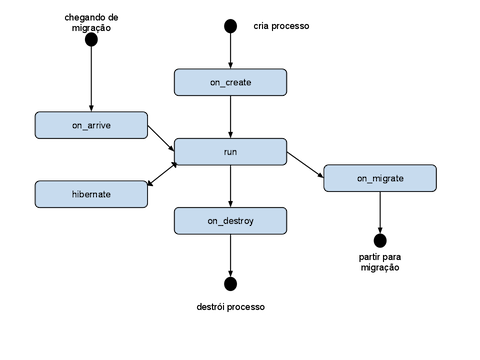
\includegraphics{estados_processos.png}}
  \caption{Ciclo de vida de um processo lógico.}
\label{fig:estados_processos}
\end{figure}

\begin{figure}
  \centerline{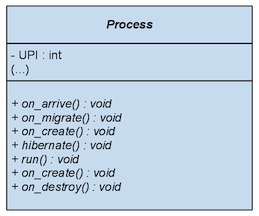
\includegraphics{process_uml.png}}
  \caption{Representação em diagrama de classe do componente \textit{process}.}
\label{fig:process_uml}
\end{figure}

Os demais métodos invocados automaticamente pelo sistema são on\_migrate, invocado antes da migração. on\_arrive, invocado assim que o processo chega no destino. hibernate, invocado quando um processo é adormecido e on\_destroy, invocado ao se destruir um processo lógico.

Naturalmente o a classe \textit{Process} comporta a criação de demais métodos além destes pré-estipulados, porém apenas estes métodos são executados de maneira automática pelo \textit{middleware} em ocasiões especiais.

\subsection{Serialização de um processo}

Serialização é a capacidade que um objeto possui de converter sua estrutura interna de dados em um formato estático, a fim de se armazenar ou reutilizar posteriormente

Um processo deve possuir a propriedade de ser serializado quando conveniente. Um processo não possui a capacidade de se serializar, ou de serializar um outro processo. O processo de serialização de um processo se dá somente a partir de chamadas internas do \textit{middleware}. Ao usuário cabe garantir que todo o código escrito seja serializável.

\section{Migração de processos \label{migracao}}

Uma das principais características propostas pelo \textit{middleware} de comunicação que compões este trabalho á a possibilidade de que processos lógicos migrem de seu nó de origem para um nó distinto no sistema. Para que isso ocorra, naturalmente, o nó destinoo deve possuir uma instância ativa de um \textit{environment} capaz de gerenciar a continuidade da vida do processo em questão.

Para que a migração ocorra, uma série de ações deve ocorrer a fim de sinalizar 

\begin{enumerate}
\item O estado do processo na tabela de endereços é modificade de Ativo para Trânsito.
\item O método on\_migrate é invocado ainda no ambiente de origem do processo.
\item O processo a ser migrado é serializado pelo \textit{environment} de origem e enviado para o ambiente de destino.
\item O ambiente de destino recebe o processo serializado e o desserializa, tornando-o um novo objeto em memória, mas mantendo os dados originais do processo.
\item O ambiente de destino atualiza o estado do processo em sua tabela local de Ausente para Inativo.
\item O ambiente de destino envia uma mensagem para o ambiente de origem indicando que o processo chegou, e qual o novo endereço físico do processo.
\item O \textit{environment} de origem atualiza o estado do processo para Ausente. Atualiza também o endereço físico do processo na tabela de endereços.
\item O processo executa o método on\_arrive no ambiente de destino.
\item O \textit{environment} muda o status do processo de Inativo para Ativo.
\item Por fim, o processo recupera todas as mensagens do buffer de mensagens do proxy de comunicação, resgatando eventuais mensagens recebidas enquanto o seu estado era Inativo.
\item O processo, já em estado ativo, executa o método run.
\item Uma mensagem em \textit{broadcast} é enviado a todos os \textit{environment}, sinalizando o novo endereço físico correspondente à aquele processo acaba de migrar. As tabelas de endereços são então atualizadas.
\end{enumerate}

Assim que o processo termina o ciclo de ações de migração ele está apto a continuar a simulação do ponto onde parou no ambiente antigo. Isto se dá poque o processo foi serializado e todos os dados foram mantidos tais como estavam instantes antes da migração.

Vale ressaltar que uma vez que esteja em processamento (executando o método run), o processo só executa a migração após o término da execução do evento em questão. Sendo assim, o método run deve ser implementado de maneira a possibilitar a preempção de eventos.

\subsection{Atualização da tabela de endereços dos processos \label{atualizacao}}

Uma vez que um processe migra de um \textit{environment} para outro, instantes após a migração apenas os dois ambientes envolvidos possuem os dados atualizados. Todo ambiente difente dos envolvidos no processo de migração possuem em suas tabelas de endereços de processos dados incorretos quanto a sua localização, portanto, enviariam mensagens para o ambiente antigo, ao qual o processo destinatário não mais pertence.

Ao receber uma mensagem de um antigo hospedeiro, um \textit{environment} (que possui o seu novo endereço), redireciona a mensagem ao proxy do ambiente que possui atualmente o processo em questão. Porém, isso inclui mais um intermediário no processo de transmissão de mensagens. Sendo assim, duas ações, em momentos distintos, são efetuadas para garantir a atualização das tabelas de endereços de processos. Primeiro, o antigo \textit{host} do processo, ao receber a mensagem, al;em de repassa-la ao atual \textit{host} também devolve uma mensagem para o remetente da mensagem, notificando-o que o endereço do ambiente que contém o processo mudou, e atualiza este endereço.

Em um momento distinto, uma segunda ação de sincronismo de tabelas é disparada. Esta ação é iniciada de forma idependente por cada \textit{environment}, enviando uma mensagem para os demais ambientes, notificando-os de quais processos lógicos encontram-se em seu poder. Isto garante uma atualização constante das diversas tabelas de endereços de processos existente na simulação.

\section{Troca de mensagens \label{troca_mensagens}}

No modelo de comunicação baseado em proxy, quando um processo deseja enviar uma mensagem a um segundo processo, a mensagem é primeiramente enviada ao proxy do \textit{environment} ao qual o processo remetente reside, e o proxy é responsável por resolver a correlação entre endereço lógico e o endereço físico, e enfim enviar a mensagem ao processo destinatário. O principal motivo de se deixar o proxy responsável pelo envio da mensage é se possibilitar que existam uma pequena quantidade de tabelas de correlação de endereços, e assim, que existam menos atualizações de tabelas em uma migração.

Em um modelo onde cada processo resolveria o envio de mensagem diretamente, a quantidade de tabelas de endereços seria proporcional à quantidade de processos (e não proporcional à quantidade de ambientes, como é na arquitetura proposta). Ao haver uma migração, existirão menos tabelas a serem atualizadas na arquitetura baseada em comunicação inter-proxies, ao passo que na comunicação direta entre processos, a quantidade de tabelas a serem atualizadas seria bem maior.

\subsection{Comunicação direta e indireta}

Quando a comunicação é feita por dois processos lógicos residentes em diferentes \textit{environments} (e por consequência, em máquinas distintas da rede) a comunicação se passa através do \textit{proxy} do \textit{environment} do remetente, e esse é responsável por enviar a mensagem ao \textit{proxy} do processo destinatário. O fluxo de comunicação é ilustrada de maneira simplificada na Figura~\ref{fig:indireta}.

Neste caso, quando ao processo P1 enviar uma mensagem ao processo P3, o próprio processo requisita diretamente ao \textit{environment} o envio da mensagem. A mensagem é então encaminha de P1 para o \textit{proxy} do seu \textit{environment} que detecta, através da tabela de endereço de processos, o endereço físico do processo alvo. 

Uma vez que a mensagem a ser enviada está em posse do \textit{proxy} do \textit{environment} destinatário, duas modalidades de comunicação podem ocorrer. A modalidade padrão é a comunicação indireta, onde o \textit{proxy} em posse da mensagem irá envia-la ao \textit{proxy} do ambiente que contém o receptor da mensagem. Uma vez que a mensagem esteja no \textit{proxy} do destinatário, este a encaminha para o processo (Figura~\ref{fig:indireta}).

Uma alternativa à comunicaçào indireta é a comunicação direta, onde o \textit{proxy} do processo de origem, uma vez obtido o endereço físico do processo destinatário, envia a mensagem diretamente para o processo receptor (Figura~\ref{fig:direta}). O método direto é útil por eliminar um intermediário na transmissão da mensagem, mas possui um inconveniente que pode anular o ganho da eliminação do intermediário. Caso haja uma migração, a mensagem não é automaticamente redirecionada para o novo ambiente em que o processo se localiza, mas sim é levantado uma excessão na comunicação, o que levaria a um tratamento de excessão, que por sua vez seria encarregado de localizar o processo em seu novo endereço físico e retransmitir a mensagem.

Cabe salientar que em caso de falha na transmissão da mensagem na modalidade de comunicação direta, a excessão levantada deve ser tratada não pelo processo, mas pelo \textit{environment}, pois a mensagem encontra-se em posse do \textit{proxy}

\begin{figure}
  \centerline{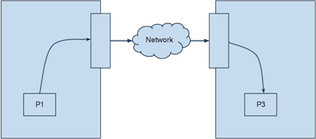
\includegraphics{Communication_indireta.png}}
  \caption{Comunicação indireta \textit{proxy-process}.}
\label{fig:indireta}
\end{figure}

\begin{figure}
  \centerline{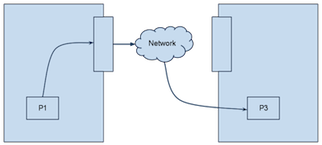
\includegraphics{Communication_direta.png}}
  \caption{Comunicação direta \textit{proxy-process}.}
\label{fig:direta}
\end{figure}

\subsection{Comunicação local direta}

Uma terceira modalidade de comunicação é a comunicação direta, via endereço físico (Figura~\ref{fig:direta_mesmo}), entre processos que habitam um mesmo ambiente. Nesta modalidade um processo que se comunica constantemente com outro processo no mesmo \textit{environment} adquire o seu endereço físico e faz a comunicação direta, sem a necessidade de se passar por um \textit{proxy} de comunicação.

Assim como na comunicação direta, neste caso há um ganho na transmissão da mensagem entre origem e destino por se excluir o \textit{proxy} como intermediário da transmissão. Entretanto, no caso de uma migração, as mensagens não seriam automaticamente redirecionadas para o processo destinatário, cabendo assim ao usuário do \textit{middleware} o tratamento de excessão caso esta aconteça.

A comunicação local direta, assim como a comunicação direta, são opções que devem ser exploradas em casos onde a migração de processos é reduzida ou nula.

\begin{figure}
  %\centerline{\includegraphics{Communication_superdirect.png}}
  \caption{Comunicação direta \textit{process-process}.}
\label{fig:direta_mesmo}
\end{figure}

\section{Serialização em grande escala} %trata da serialização de um environment ou até mesmo da simulação como um todo
\section{Comunicação grupal} % mensagens em multicast
\section{Migraçoes em grande escala e migrações de ambientes \label{migra_ambiente}} %casos de excessão
		%% 4 Proposta de arquitetura para simulação distribuída
\chapter{Arquitetura do \textit{framework} de simulação}

Uma vez definida a arquitetura de \textit{middleware} de comunicação a ser utilizado durante este projeto, o próximo passo é a definição do funcionamento e da arquitetura da camada de simulação, aqui genericamente denominado \textit{framework}.

Esta camada, conforme ilustrada na figura~\ref{fig:camada_central}, compreende diversos sub-componentes do framework (aqui esses sub-componentes serão denominados genericamentes de módulos, para que se distingua dos componentes, objetos utilizados para descrever um modelo a ser simulado). Cada módulo que compreende o kernel se liga ao módulo central, denominado \textit{kernel}. Este é o responsável por coordenar a simulação, aplicando sincronização e balanceamento de carga, além de gerenciar o ciclo de vida da simulação (quando começar, quando terminar, etc).

\begin{figure}
  \centerline{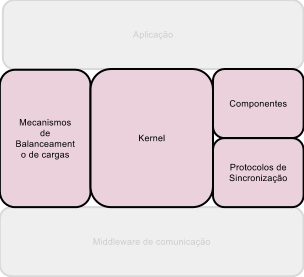
\includegraphics{camada_framework.png}}
  \caption{A camada aqui denominada \textit{framework}.}
\label{fig:camada_central}
\end{figure}

\section{O módulo Componente}

Um componente é uma abstração de um comportamento que desejamos reproduzir na nossa simulação. Na abstração de um sistema de caixa de supermercados, por exemplos, pode-se extrair três componentes (que são comuns em muitas situações na simulação de eventos discretos): o produtor, a fila de espera e o consumidor.

Uma biblioteca de componentes deve proporcionar objetos parametrizáveis que permitam a descrição do comportamento de cada um deles. No caso citado anteriormente, o componete produtor deve suportar parâmetros que, por exemplo, descreva a taxa de criação de novos evento, e as características de cada evento criado.

Os componentes são construidos diretamente em cima do objeto \textit{process} da camada de comunicação. Isso garante ao componente criado, por herança direta, toda funcionalidade de comunicação entre outros componentes. Desta maneira, basta ao usuário do framework descrever na modelagem qual a conexão que cada componente faz, que esta é reproduzida automaticamente pelo framework, independente se esses componentes são processo cohabitantes ou não-cohabitantes.

Em alguns casos é conveniente que componentes sejam combinados a fim de que um novo componente seja criado. Uma das justificativas seria, por exemplo, garantir que doi componentes primitivos se comportem como um único compoente, evitando assim que estes sejam por ventura separados e passem a cohabitar ambientes diferentes. Em um exemplo, é conveniente que o um componente do tipo fila, que tem como características armazenar eventos que serão consumidos por um componente do tipo consumidor, seja encapsulado junto ao seu consumidor.

\section{Componentes básicos}

O tipo primitivo de um componente no \textit{framework} proposto é desenvolvido em cima da classe \textit{process} (conforme ilustrado na figura~\ref{fig:basic_component}) e deve ser capaz de proporcionar alguns elementos básicos de fluxo de eventos como por exemplo um (ou diversos) canais de entrada de eventos, ambiente de processamento e canais de saída de eventos.

\begin{figure}
  \centerline{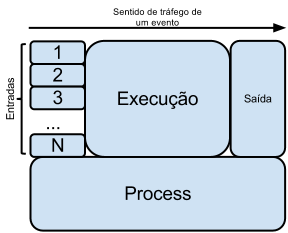
\includegraphics{basic_component.png}}
  \caption{Arquitetura básica de um componente primitivo.}
\label{fig:basic_component}
\end{figure}

\begin{figure}
  \centerline{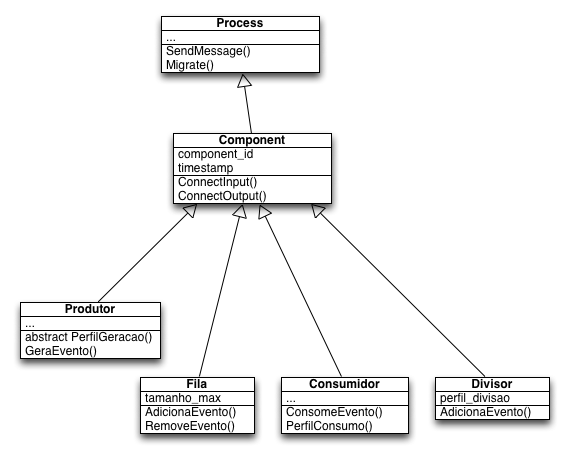
\includegraphics{uml_componentes.png}}
  \caption{Hierarquia dos componentes básicos.}
\label{fig:uml_components}
\end{figure}

Sobre este componente primitivo são construídos quatro componentes básicos(Figura~\ref{uml_components}), suficientes para demonstrar a implementação de alguns modelos para simulação. Estes componentes são: fila, gerador, consumidor e divisor.

Cada um desses componentes é construído sobre a arquitetura do componente primitivo descrito na seção~\ref{primitivo}. Por motivos naturais, nem todos os componentes implementos esse modelo em sua totalidade. Componentes como os geradores de eventos, por exemplo, não possuem canais de entrada de eventos, uma vez que a sua função é a de apenas gerar novos eventos com base em uma parametrização de suas características para que se comporte conforme o modelo que descreve suas ações. 

\subsection{O componente Fila}

A fila é o o ponente responsável por armazenar eventos, ordenando-os com base no seu \textit{timestamp}. Cada evento que chega à fila é alocado respeitando a ordem referente ao seu \textit{timestamp}, e cada vez que um elemento é retirado da fila, isto é feito retirando-se o primeiro elemento da fila, ou seja, o elemento com o menor \textit{timestamp}. 

A fila é um componente passivo, ou seja, ela não executa nenhum tipo de ação sobre os eventos nela existente. Por ser um componente passivo, é o componente gerador que deve executar a ação de inserir um novo evento na fila, e é um componente consumidor que deve executar a ação de retirar o evento de menor \textit{timestamp} da fila.

Uma das características mais importantes do componente fila é o seu tamanho. Uma fila pode ou não ter um tamanho definido, porém uma vez definido um tamanho para esta fila, quando este tamanho se excede, ou seja, quando a quantidade de eventos inseridos cresce em uma velocidade tão grande que o consumidor atrelado àquela fila não consegue consumi-los em tempo hábil podem ocorrer dois eventos, dependendo de como o usuário do framework descreveu em seu modelo. No caso mais simples o usuário determina que ao se exceder a quantidade de elementos em uma fila, uma excessão do tipo QueueOverflow() seja lançada, e a simulação se encerra.

Em um caso mais elaborado, ao se atingir o limite de uma fila esta pode apenas negar a inserção de novos elementos até que haja espaço suficiente. Neste caso, há uma propagação da condição de estacionamento da execução para os elementos atrelados à essa fila, causando um efeito que reflete em grande parte do sistema. 

\begin{figure}
  \centerline{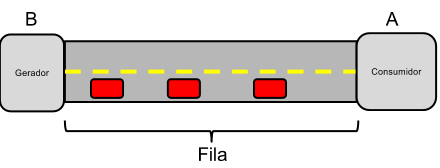
\includegraphics{cruzamento.png}}
  \caption{Modelagem de uma via urbana.}
\label{fig:cruzamento}
\end{figure}

Um exemplo típico que ilustra esse caso é a simulação de uma sequência de cruzamentos em uma via urbana, ilustrada na Figura~\ref{fig:cruzamento}. A quantidade de carros que cabem em um intervalo entre os dois cruzamentos A e B é finito, e se o cruzamento A não consome carros em uma velocidade maior ou igual à que eles chegam, há um crescimento na quantidade de carros entre os dois cruzamentos, o que pode levar à paralização temporária da simulação, até que o consumidor A consuma eventos, liberando espaço na fila.

\subsection{O componente Gerador}

Assim como ilustrado na Figura~\ref{fig:cruzamento}, um exemplo de gerador de eventos é uma extremidade de uma via de trânsito, que gera eventos (no exemplo citado, carros) em uma determinada taxa de tempo, com uma determinada frequência.

Um dos comportamentos parametrizáveis do componente gerador é a função que modela a taxa de criação de novos eventos ao longo do tempo. Um sistema que se deseja maior fidelidade quanto aos dados simulados deve permitir uma detalhada parametrização do comportamento de seus componentes. Neste \textit{framework} isto é feito através das funções geradoras, que são funções que recebem como parâmetros dados da simulação e resultam em decisões sobre a criação ou não de novos eventos, e o comportamento desses eventos.

Mais detalhes sobre o funcionamento das funções geradoras são abordados na seção~\ref{funcoes_geradoras}.

\subsection{O componente Consumidor}

Assim como o componente gerador, o componente consumidor é parametrizável através de funções externas que descrevem o seu comportamento ao longo do tempo de simulação. Outros dados levados em conta durante a execução de um evento por um consumidor são as características internas dos eventos.

O componente gerador possui múltiplas entradas de dados, porém apenas um canal de saída. Uma saída do gerador pode ser dividida em várias utilizando um componente divisor(\ref{divisor}). A razão de se adotar este \textit{design} de um único canal de saída e múltiplas entradas se justifica pela simplicidade da arquitetura do modelo, uma vez que o componente gerador não precisaria se encarregar do comportamento que os eventos por ele processados tomariam após o processamento.

\begin{figure}
  \centerline{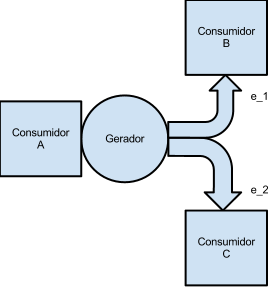
\includegraphics{gerador_mais_consumidor.png}}
  \caption{Um processo consumidor que gera eventos. No caso ilustrado, o consumidor A gera, através de um componente Gerador, simultaneamente os eventos e\_1 e e\_2 que são então encaminhados para os consumidores B e C}
\label{fig:multiple_sons}
\end{figure}

Uma vez que o evento é processado por um consumidor, este pode tomar três caminhos distintos: o evento pode simplesmente morrer, o evento pode ser redirecionado para um novo processador (ou mesmo para o mesmo processador, dependendo da necessidade da simulação), porém com suas características originais mantidas. Uma terceira possibilidade é que o evento sofra uma modificação nas suas características antes de ser encaminhado a diante.

Em condições especiais, um componente processador pode ser conectado à um gerador, e a ação de executar um evento poderia gerar um ou mais eventos distintos por esse gerador, que seriam então inseridos no sistema. Um exemplo prático desta aplicação é a simulação do fluxo de trabalho de uma companhia, onde a chegada de um documento pode disparar duas tarefas diferentes a serem feitas em paralelo (Figura~\ref{fig:multiple_sons}).


\subsection{O componente Divisor \label{divisor}}

Um componente divisor possui multiplas entradas e múltiplos canais de saída. A sua função é, dado um evento e que entra pelo divisor, aplicar uma função de decisão que mapeie este evnto para uma de suas saídas.

Assim como os componentes consumidor e gerador, o comportamento de um divisor é parametrizável através de funções que descrevem o seu comportamento com base nas características do modelo simulado.

A aplicação mais comum de um divisor é atrelado à saída de um processador, ou de um gerador, a fim de o evento que é entregue a ele seja redirecionado a um caminho aleatório, porém descrito por sua função de comportamento.

\section{O \textit{kernel} do \textit{framework}}

A parte central do \textit{framework} desenvolvido neste trabalho aqui é ilustrada pelo blog \textit{kernel} (Figura~\ref{camada_central}). O \textit{kernel} é o responsável por gerenciar a simulação, incrementando o \textit{timestep} de cada componente, e tomando decisões de migração, comunicação, sincronismo e balanceamento de carga.

Para realizar tais funções o kernel se apoia diretamente no \textit{middleware} de comunicação descrito no capítulo~\ref{chapter_middleware}, além de utilizar os algorítmos de balanceamento de carga e os protocolos de sincronismo da simulação.

A cada incremento discreto da simulação, denominado \textit{timestep}, o kernel do \textit{framework} realiza as seguintes funções:

\begin{itemize}
\item Incrementar o \textit{timestamp} de cada componente.
\item Verificar se existem mensagens no \textit{buffer} do middleware, e tentar redireciona-las ao destinatário.
\item Verificar, através do módulo de balanceamento de cargas, se existem processos que devem ser migrados.
\item Verificar, através do módulo de sincronismo, se ocorreram mensagens \textit{straggler}. Caso afirmativo, designa ao módulo de sincronismo a tarefa de re-sincronizar o sistema.
\item Gerencia, através do módulo de sincronismo, as tarefas de salvamento de estados.
\end{itemize}

O \textit{kernel} do sistema executa estes processos em \textit{loop} até que o números de iterações previstas acabe, ou até que a simulação seja interrompida por algum evento externo.

\section{Protocolos de sincronização}

Uma das premissas do projeto é a possibilidade de se substituir certos módulos do framework conforme a necessidade do seu usuário. Este encapsulamento de certas funcionalidades do \textit{framework} possibilita uma facilidade quando se deseja trocar algum componente do sistema.

Para que isto seja possível, o \textit{kernel} do sistema deve garantir uma \textit{interface} de acessos a diveras funções e variáveis do ambiente, permitindo assim que o módulo adquira dados referentes à simulação e interfira no seu funcionamento.

No caso da sincronização dos processos, o módulo em questão deve ser capaz de adquirir valores como o \textit{LVT} e o \textit{GVT}, idendtificar mensagens \textit{straggler}, além de ter acesso ao \textit{middleware} de comunicação para trocar mensagens com os demais nós do sistemas, e requerer o \textit{rollback} para um determinado \textit{timestamp}.

\section{Algoritmos de balanceamento de carga}

Assim como no caso dos protocolos de sincronização de eventos, os algorítmos de balanceamento de cargas do sistema também são modularidos e podem ser trocados pelo usuário (ou até mesmo customizados).

Cabe ao \textit{framework} prover uma interface que possibilite ao módulo de balanceamento requerere ao \textit{kernel} informações sobre a carga de cada nó do sistema, tal qual o perfil de comunicação de cada \textit{process}. Com base nesses dados, o algorítmo decide qual processo deve ser migrado, e para qual máquina.

Para que a migração seja possível, o \textit{kernel} deve prover mecanismos para que o módulo de balanceamento de cargas requira a migração de um determinado processo.
      %% 5 Framework desenvolvido para sustentar a arquitetura
\chapter{Implementação}

\chapter{Discussões finais e Conclusões}

               %% Conclsões e trabalhos futuros
\include{biblio}
% \chapter{A linguagem \textit{Python} \label{appendix_python}}
\chapter{Diagrama de classes \label{appendix_uml_completo}}
\chapter{Distribuiçao}

O projeto \textit{framework} desenvolvido neste trabalho recebeu o nome de T100. O projeto T100, incluindo seu código fonte e toda a documentação é distribuído sobre licensa \textit{GPL - General Public License}, que dá ao seu usuário garantias de liberdade para uso, modificação e redistribuição do software como um todo, incluindo o seu código fonte.

\section{Licensa}

O projeto T100 é distribuído sobre licensa \textit{GPL v3.0}.

\subsection{\emph{License}}

\lstinputlisting[label=license,
                 caption="Licensa de uso do software"]{license.txt}

\subsection{Informações sobre a licensa}

Para mais informações sobre a lincesa \textit{GPL v3.0} visite:

http://www.gnu.org/licenses/gpl.html

\section{Disponibilidade}

O código fonte, junto aos exemplos de uso e documentação deste projeto, podem ser adquiridos através do endereço:

http://github.com/alvesjnr/T100


\chapter{Árvore de diretórios \label{appendix_tree}}

\lstinputlisting[language=Python,
                 label=source_tree,
                 caption="Árvore de diretórios do projeto."]{source_tree.txt}

\chapter{Classe com método assíncrono \label{appendix_proxy_example}}

\lstinputlisting[language=Python,
                 label=proxy_example,
                 caption="Exemplo de chamada de métodos assíncronas na classe \textit{Proxy}"]{proxy_example.py}
% ----------------------------------------------------------------
\bibliographystyle{abnt-alf}
\bibliography{biblio}             %% REFERENCIAS (deve-se possuir o arquivo do tipo bibitex)
% ----------------------------------------------------------------
\end{document}
% ----------------------------------------------------------------
